\documentclass[a4paper,10pt]{article}
\usepackage[UTF8]{ctex}
\usepackage{geometry}
\usepackage{tikz}
\usetikzlibrary{shapes.geometric, arrows.meta, positioning, calc, trees}
\usepackage{longtable}
\usepackage{array}
\usepackage{fancyhdr}
\usepackage{xcolor}
\usepackage{amsmath}
\usepackage{amssymb}
\usepackage{hyperref}
\geometry{left=2.5cm, right=2.5cm, top=3cm, bottom=2.5cm}
\pagestyle{fancy}
\fancyhf{}
\fancyhead[C]{\small computeObstacleAffineConstraint 函数设计文档}
\fancyfoot[C]{\thepage}
\setcounter{secnumdepth}{3}
\setcounter{tocdepth}{3}
\tikzset{
    startstop/.style={ellipse, draw, fill=red!10, text width=8em, minimum height=0.9cm, align=center},
    process/.style={rectangle, draw, fill=blue!5, text width=11em, minimum height=1.1cm, align=center},
    decision/.style={diamond, draw, fill=green!10, text width=7em, minimum height=1cm, align=center},
    arrow/.style={thick,->,>=Stealth}
}
\begin{document}
\begin{titlepage}
    \centering
    {\Huge\textbf{computeObstacleAffineConstraint（单障碍物 HOCBF 仿射约束生成）函数设计}\par}
    \vspace{1.5cm}
    \renewcommand{\arraystretch}{1.5}
    \begin{tabular}{|l|l|l|l|}
        \hline
        文件密级 & 内部公开 & 编号 & CBF-DOC-COMPUTEOBSTACLEAFFINECONSTRAINT \\ \hline
        版本 & V1.0 & 内容 & computeObstacleAffineConstraint（单障碍物 HOCBF 仿射约束生成）函数设计 \\ \hline
        设计 & 许庆 & 联系方式 & 18612426814 / qingxu@tsinghua.edu.cn \\ \hline
        审核 & - & 审批 & - \\ \hline
        发布日期 & 2026 年 6 月 26 日 & & \\ \hline
    \end{tabular}
    \vspace{1.5cm}
    \section*{文件更改记录}
    \begin{longtable}{|c|c|p{4cm}|c|c|c|c|}
        \hline
        日期 & 版本号 & 修订说明 & 辅助AI & 修订 & 审核 & 审批 \\ \hline
        2026-6-26 & V1.0 & 初次设计 & Claude-Opus-4.7 & 许庆 & - & - \\ \hline
    \end{longtable}
\end{titlepage}
\tableofcontents
\newpage
\section{公有函数设计}
\subsection{computeObstacleAffineConstraint（单障碍物 HOCBF 仿射约束生成）函数设计}
\subsubsection{函数需求}
\par 本函数实现 \textbf{单障碍物 HOCBF 仿射约束生成}。其在 CBF 自动驾驶安全控制流水线中承担如下职责：整合 B、dotB、ddBFree，生成形如 betaA*a + betaT*tan($\textbackslash{}delta$) >= bound 的仿射约束。
\par 头文件路径：\texttt{include/cpp/computeObstacleAffineConstraint/computeObstacleAffineConstraint.hpp}；源文件路径：\texttt{src/cpp/computeObstacleAffineConstraint/computeObstacleAffineConstraint.cpp}。
\subsubsection{算法设计}
\par 本函数核心数学表达式如下：
\begin{equation}
\beta_a a + \beta_t \tan\delta_f \geq -\bigl(\ddot B|_{free} + (\alpha_1+\alpha_2)\dot B + \alpha_1\alpha_2 B\bigr)
\end{equation}
\par 实现步骤：
\begin{enumerate}
  \item \textbf{call\_b}: 调用 computeBarrierSquared 求 B
  \item \textbf{call\_dotb}: 调用 computeBarrierFirstDerivative 求 dotB
  \item \textbf{call\_ddb}: 调用 computeBarrierSecondDerivativeFree 求 ddBFree
  \item \textbf{coef}: betaA=-2dx, betaT=-2 v\textasciicircum{}2/L * dy
  \item \textbf{bound}: bound = -(ddBFree+($\textbackslash{}alpha$1+$\textbackslash{}alpha$2)dotB+$\textbackslash{}alpha$1$\textbackslash{}alpha$2 B)
\end{enumerate}
\subsubsection{程序流程图}
\begin{figure}[h]
    \centering
    \begin{tikzpicture}[node distance=1.6cm]
    \node (start) [startstop] {开始};
    \node (p0) [process, below of=start, yshift=-0.3cm] {调用 computeBarrierSquared 求 B};
    \node (p1) [process, below of=p0, yshift=-0.3cm] {调用 computeBarrierFirstDerivative 求 dotB};
    \node (p2) [process, below of=p1, yshift=-0.3cm] {调用 computeBarrierSecondDerivativeFree 求 ddBFree};
    \node (p3) [process, below of=p2, yshift=-0.3cm] {betaA=-2dx, betaT=-2 v\textasciicircum{}2/L * dy};
    \node (p4) [process, below of=p3, yshift=-0.3cm] {bound = -(ddBFree+($\textbackslash{}alpha$1+$\textbackslash{}alpha$2)dotB+$\textbackslash{}alpha$1$\textbackslash{}alpha$2 B)};
    \node (end) [startstop, below of=p4, yshift=-0.3cm] {返回 / 写回输出};
    \draw [arrow] (start) -- (p0);
    \draw [arrow] (p0) -- (p1);
    \draw [arrow] (p1) -- (p2);
    \draw [arrow] (p2) -- (p3);
    \draw [arrow] (p3) -- (p4);
    \draw [arrow] (p4) -- (end);

    \end{tikzpicture}
    \caption{computeObstacleAffineConstraint 函数程序流程图}
    \label{fig:flow_computeObstacleAffineConstraint}
\end{figure}
\subsubsection{函数接口}
\par 输入参数列表：
\begin{itemize}
  \item \texttt{egoVelocity} (double) -- 自车速度 v
  \item \texttt{wheelBase} (double) -- 轴距 L
  \item \texttt{alpha1} (double) -- HOCBF 一阶系数 $\textbackslash{}alpha$1
  \item \texttt{alpha2} (double) -- HOCBF 二阶系数 $\textbackslash{}alpha$2
  \item \texttt{obstacle} (ObstacleState) -- 障碍物 ego-frame 状态
  \item \texttt{axObEgo} (double) -- 障碍物 ego-frame 加速度 x
  \item \texttt{ayObEgo} (double) -- 障碍物 ego-frame 加速度 y
  \item \texttt{safetyRadius} (double) -- 安全半径
\end{itemize}
\par 输出参数列表：
\begin{itemize}
  \item \texttt{return} (AffineConstraint) -- {betaA, betaT, bound}
\end{itemize}
\subsubsection{输入输出模块图}
\begin{figure}[h]
    \centering
    \begin{tikzpicture}[>=Stealth]
        \node[draw, rectangle, minimum width=4.5cm, minimum height=2cm, fill=blue!5] (func) at (0,0) {\large{\textbf{computeObstacleAffineConstraint}}};
        \draw[->, thick] (-3.5,0.4) -- node[above]{I (输入)} (-2.3,0.4);
        \draw[->, thick] (2.3,0.4) -- node[above]{O (输出)} (3.5,0.4);
        \draw[->, thick] (0,-1.0) -- node[right]{f (返回)} (0,-2.0);
    \end{tikzpicture}
    \caption{computeObstacleAffineConstraint 函数输入输出模块图}
    \label{fig:io_computeObstacleAffineConstraint}
\end{figure}
\subsubsection{函数诸元表}
\begin{table}[h]
    \centering
    \caption{computeObstacleAffineConstraint 函数诸元表}
    \label{tab:meta_computeObstacleAffineConstraint}
    \begin{tabular}{|c|c|c|c|c|}
        \hline
        中文名 & 英文名 & 性质 & 级别 & 入库 \\ \hline
        单障碍物 HOCBF 仿射约束生成 & computeObstacleAffineConstraint & 组件 & 应用层 & 是 \\ \hline
    \end{tabular}
\end{table}
\subsubsection{函数架构}
\begin{figure}[h]
    \centering
    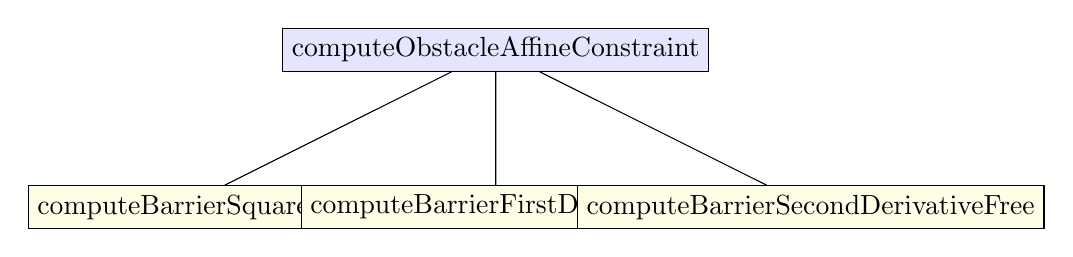
\begin{tikzpicture}[>=Stealth, level distance=2cm,
        level 1/.style={sibling distance=4cm}]
        \node[draw, fill=blue!10] {computeObstacleAffineConstraint}
        child {node[draw, fill=yellow!10] {computeBarrierSquared}}
        child {node[draw, fill=yellow!10] {computeBarrierFirstDerivative}}
        child {node[draw, fill=yellow!10] {computeBarrierSecondDerivativeFree}}
        ;
    \end{tikzpicture}
    \caption{computeObstacleAffineConstraint 函数架构图}
    \label{fig:arch_computeObstacleAffineConstraint}
\end{figure}
\subsubsection{下级函数需求}
\begin{itemize}
  \item \texttt{computeBarrierSquared}：B 值
  \item \texttt{computeBarrierFirstDerivative}：dotB
  \item \texttt{computeBarrierSecondDerivativeFree}：ddBFree
\end{itemize}

\subsubsection{测试用例表}
\noindent\textbf{正常场景测试用例如表~\ref{tab:normal_computeObstacleAffineConstraint} 所示：}
\begin{table}[h]
\centering
\caption{computeObstacleAffineConstraint 正常场景测试用例}
\label{tab:normal_computeObstacleAffineConstraint}
\begin{tabular}{|c|p{3.5cm}|p{3.5cm}|p{3.5cm}|}
\hline
ID & 描述 & 输入 & 期望输出 \\ \hline
  TC1 & 正常用例 1 & 见 cases.json & 见 cases.json \\ \hline
  TC2 & 正常用例 2 & 见 cases.json & 见 cases.json \\ \hline
  TC3 & 正常用例 3 & 见 cases.json & 见 cases.json \\ \hline
  TC4 & 正常用例 4 & 见 cases.json & 见 cases.json \\ \hline
  TC5 & 正常用例 5 & 见 cases.json & 见 cases.json \\ \hline
\end{tabular}
\end{table}

\noindent\textbf{异常场景测试用例如表~\ref{tab:abnormal_computeObstacleAffineConstraint} 所示：}
\begin{table}[h]
\centering
\caption{computeObstacleAffineConstraint 异常场景测试用例}
\label{tab:abnormal_computeObstacleAffineConstraint}
\begin{tabular}{|c|p{3.5cm}|p{3.5cm}|p{3.5cm}|}
\hline
ID & 描述 & 输入 & 期望输出 \\ \hline
  EC1 & NaN 输入 & 任一标量=NaN & 输出含 NaN \\ \hline
  EC2 & Inf 输入 & 任一标量=Inf & 输出含 Inf \\ \hline
  EC3 & 数学边界 & 极限值 & 结果有界或返回 false \\ \hline
  EC4 & QP 不可行 & 约束相互冲突 & 返回 feasible=false \\ \hline
\end{tabular}
\end{table}

\noindent\textbf{符号说明：}
\begin{itemize}
  \item dx, dy: ego-frame 相对位置 (m)
  \item v\_rx, v\_ry: ego-frame 相对速度 (m/s)
  \item r: 安全圆半径 (m)
  \item B: Barrier 函数值
\end{itemize}
\end{document}
